\section{Experiments}
\label{sec:experiments}


This section provides information about computational experiments, their configuration, results and details
of implementation.

Code for experiments has been developed on \texttt{Python 3.8} using \texttt{Pytroch Geometric} framework
\footnote{\url{https://pytorch-geometric.readthedocs.io/en/latest/index.html}}
\cite{PyG}.
This frameworks contains a lot of implemented graph neural network models,
provides a convenient tools to operate data and suggests an algorithm to train and validate models.

Below there are description of the data preparation process, followed by model implementation details and description
of the organization of the training process.


% TODO: say about what experiments are

\subsection{Data preparing process}

Framework \texttt{Pytorch} proposes a unified way to work with data.
It consists of two stages:
preapre dataset object with defined <TODO check from doc> methods to access data and configure DataLoader<TODO linK>
to form batch of predefined size. Batch consists of vectors of features from datasets and labels corresponding them
in the case of solving the classification problem. <TODO: edit> . DataLoader allows to
itearete data within one train epoch.

The same approach is used in \texttt{Pytroch Geometric} geometric framework. The difference is that
dataset object should implenet special interface <TODO>, and DataLoaders allows to union several graph in single batch.

% TODO about minibatchin
% Since graphs in graph classification datasets are usually small, a good idea is to batch the graphs before inputting them into a Graph Neural Network to guarantee full GPU utilization. In the image or language domain, this procedure is typically achieved by rescaling or padding each example into a set of equally-sized shapes, and examples are then grouped in an additional dimension. The length of this dimension is then equal to the number of examples grouped in a mini-batch and is typically referred to as the batch_size.

% However, for GNNs the two approaches described above are either not feasible or may result in a lot of unnecessary memory consumption. Therefore, PyTorch Geometric opts for another approach to achieve parallelization across a number of examples. Here, adjacency matrices are stacked in a diagonal fashion (creating a giant graph that holds multiple isolated subgraphs), and node and target features are simply concatenated in the node dimension:

% TODO: batching picture


In this work two groups of datasets are used. The first one contains datasets from TUdataset\cite{TUDataset}
collection: MUTAG, PROTEINS, DD and ENZYMES. \texttt{Pytroch Geometric} provides convenient access to all of then with

\texttt{torch\_geometric.datasets.TUDataset} class.
\footnote{\url{https://pytorch-geometric.readthedocs.io/en/latest/modules/datasets.html\#torch_geometric.datasets.TUDataset}}


The second group contains of Brain fMRI dataset and Kidney RNASeq dataset used in \cite{Netpro2vec}. Graphs from
these datasets are available in \texttt{graphml} format. So to operate them in the way
defined in \texttt{torch\_geometric.datasets}, there has been developed a custom \texttt{Dataset} object, which
extend \texttt{InMemoryDataset} \footnote{\url{https://pytorch-geometric.readthedocs.io/en/latest/modules/data.html\#torch_geometric.data.InMemoryDataset}}
class and allows to process them the same way as datasets from the first group.

\subsection{Models configuration}

Three graph neural networks are trained and inferenced in the current work. Below there are information
about these models' configuration used in exeriments.

GCN model contains 3 convolution layers with hidden layer dimension equal to $128$,
one hidden layer with dimension $64$ and the final linear layer to calculate logits.
The valus of hyperparameters are the following: $\alpha=0.5$ and $\lambda=0.1$.

GAT model contains two GAT convolution with 8 and 1 heads respectively and hidden deminsion equal to $64$
and linear layer with dimension $32$, followed by  final linear layer to calculate logits.

GCNII model contains of $16$ convolutions with hidden size $64$,  linear layer with dimension $32$,
followed by  final linear layer to calculate logits.


\subsection{Models training pipeline}


To train and evaluate model there has been prepared the following pipeline.

Firstly, dataset prepared and uploaded to \texttt{Google Drive}. Then code for training is wrapped
into command line util and pushed to \texttt{GitHub} repository. Training and evaluation process run
in \texttt{Google Colab}.Training metrics are uploaded to \texttt{Weight And Biasis} - application for displaying
and storing graphs in runtime. Testing metrics are uploaded to \texttt{Google Drive}.
The whole pipeline is shown on figure \ref{fig:pipeline}. Example of graph on  \texttt{Weight And Biasis}
are shown on figure \ref{fig:wnb}

\begin{figure}[t]
    \centering
    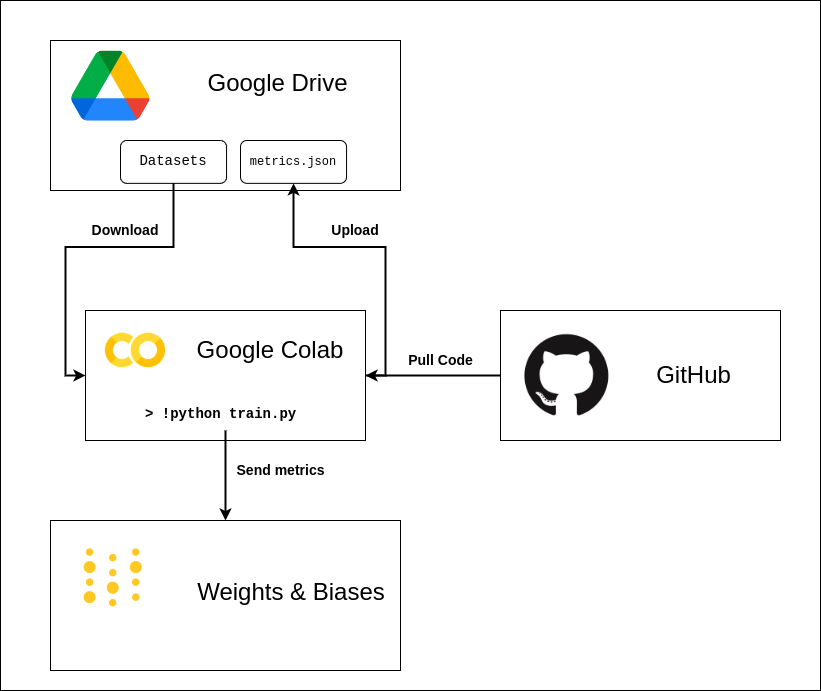
\includegraphics[width=0.7\textwidth]{schema}
    \caption{Training pipeline schema}
    \label{fig:pipeline}
\end{figure}


\begin{figure}[h]
    \centering
    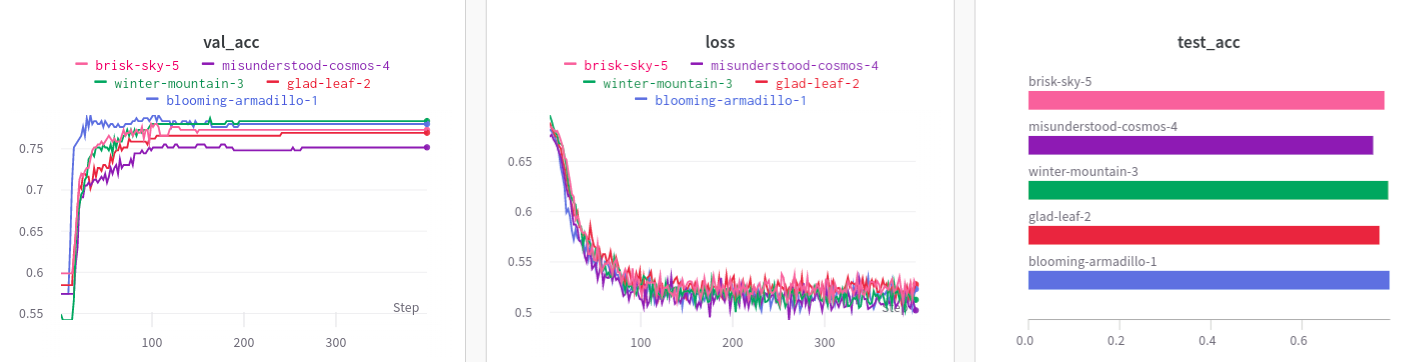
\includegraphics[width=1\textwidth]{wnb}
    \caption{Graphs example from Weight And Biasis. Graps are drawing in training runtime}
    \label{fig:wnb}
\end{figure}

\subsection{Node features transformation}

% about node features

% TODO: move this section from here?

All neural networks models, which are  <TODO>... requires node feature matrix. This matrix
acts a a signal in term of signal processing with convolutions and the base embeddings of nodes,
which transformation should be applied to.

In some cases, encoded node labels may be used as node features. However, some networks
do not have neither node labels, nor features.
In that case, node features can be constructed additionaly as a preprocessing step.

In the current work two approches will be used to constuct node features.

The first one is to use one-hot reprosentation of node degrees. So the node features matrix
is matrix $X \in \{0,1\}^{N \times d}$ having property $\sum_{j=1}^{d}X_{ij} = 1$ for any $i \in 1 \dots N$,
where $N$ is the number of nodes in graph $G$ and $d$ is max degree over all nodes in graph.

% TODO: схемку с примером

The second approach is to use Node Distance Distribution matrix presented in \cite{Netpro2vec}.

% TODO: describe NDD matrix

% TODO: add schema

% About implementation

% Node features matrix constuction is implemented using TORCH_GEOMETRIC.TRANSFORMS package in Pytorch Geometric Framework

Node features matrix constuction is implemented using

\texttt{torch\_geometric.transforms} \footnote{\url{https://pytorch-geometric.readthedocs.io/en/latest/modules/transforms.html}}
package. It allows to apply transformation to feature matrix by concatenating or replacing current matrix with a new one.

One-hot encoded degrees features are added using built-in transformation

\texttt{OneHotDegree}
\footnote{\url{https://pytorch-geometric.readthedocs.io/en/latest/modules/transforms.html\#torch_geometric.transforms.OneHotDegree}}

Encoded degrees were concatenated to the current node labels features.

To use node distance matrix as a node feature matrix, new custom transformation was developed.


\subsection{Experiments set up}

% what should be done



\subsection{Results}

Computational experiments includes training chosen graph neural network models on different datasets with two different
Node feature matrices: one hot encoded degree matrix and node distance distribution matrix.

Accuracy is measured as mean of 5 separate runs, which include training dataset on train set, choosing
best model using validation set and evaluate accuracy on test set, which is not used during train step.
Based on these test accuracy metric, mean and standard deviation is measured.

Table \ref{tab:results} shows the result of experiments. For each model there are two types of result: "deg" and "ndd".
Model marked with "deg" uses one hot encoded node degrees as a feature matrix, while "ndd" mark stands for NDD matrix 
as a feature matrix.

\begin{table}[]
    \scriptsize
    \begin{tabular}{|c|c|c|c|c|c|c|c|}
        \hline
                               &     & MUTAG                 & PROTEINS               & ENZYMES                & DD                    & Brain fMRI             & Kidney RNA Seq        \\ \hline
        \multirow{2}{*}{GCN}   & deg & \textbf{0.884$\pm$0.043} & \textbf{0.7468$\pm$0.011} & \textbf{0.3458$\pm$0.038} & 0.756$\pm$0.01           & 0.56$\pm$0.0442           & 0.5583$\pm$0.032         \\
                               & ndd & 0.844 $\pm$ 0.037         & 0.7371$\pm$0.016          & 0.3$\pm$0.019             & \textbf{0.795$\pm$0.009} & 0.4667$\pm$0.084          & 0.5611$\pm$0.066         \\ \cline{1-8}
        \multirow{2}{*}{GAT}   & deg & 0.687$\pm$0.045          & 0.6524$\pm$0.04           & 0.2667$\pm$0.044          & 0.7128$\pm$0.018         & \textbf{0.6067$\pm$0.044} & 0.5306$\pm$0.034         \\
                               & ndd & 0.853$\pm$0.033          & 0.7206$\pm$0.019          & 0.2639$\pm$0.038          & 0.7936$\pm$0.005         & 0.5767$\pm$0.05           & \textbf{0.5639$\pm$0.04} \\ \cline{1-8}
        \multirow{2}{*}{GCNII} & deg & 0.733$\pm$0.034          & 0.6996$\pm$0.03           & 0.2889$\pm$0.03           & 0.6929$\pm$0.023         & 0.58$\pm$0.093            & 0.475$\pm$0.087          \\
                               & ndd & 0.7156$\pm$0.029         & 0.7393$\pm$0.023          & 0.2333$\pm$0.038          & 0.7766$\pm$0.013         & 0.52$\pm$0.134            & 0.5556$\pm$0.049         \\ \hline
    \end{tabular}
    \caption{Experiments results}
    \label{tab:results}
\end{table}

As result shows, that for all chosen TU Datasets, GCN model shows the best result. Accuracy of models trained and tested on one hot encoded degree feature matrices
are is higher then one on NDD matrix, except accuracy of tests on DD dataset.

Tests on datasets "Brain fMRI" and "Kidney RNA Seq" show rather low accuracy. The best accuracy for "Brain fMRI" shows GAT model with encoded degrees matrix. 
The best accuracy for "Kidney RNA Seq" shows GAT model with NDD matrix. 
